%%% Econ711: Microeconomics I
%%% Fall 2020
%%% Danny Edgel
%%%
% Due on Canvas Monday September 21, 11:59pm Central Time
%%%

%%%
%							PREAMBLE
%%%

\documentclass{article}

%%% declare packages
\usepackage{amsmath}
\usepackage{amssymb}
\usepackage{array}
\usepackage{bm}
\usepackage{changepage}
\usepackage{centernot}
\usepackage{graphicx}
\usepackage{fancyhdr}
	\fancyhf{} % sets both header and footer to nothing
	\renewcommand{\headrulewidth}{0pt}
    \rfoot{Edgel, \thepage}
    \pagestyle{fancy}
	
%%% define shortcuts for set notation
\newcommand{\N}{\mathbb{N}}
\newcommand{\Z}{\mathbb{Z}}
\newcommand{\R}{\mathbb{R}}
\newcommand{\Q}{\mathbb{Q}}
\newcommand{\lmt}{\underset{x\rightarrow\infty}{\text{lim }}}
\newcommand{\neglmt}{\underset{x\rightarrow-\infty}{\text{lim }}}
\newcommand{\zerolmt}{\underset{x\rightarrow 0}{\text{lim }}}
\newcommand{\usmax}{\underset{1\leq k \leq n}{\text{max }}}

%%% define column vector command (from Michael Nattinger)
\newcount\colveccount
\newcommand*\colvec[1]{
        \global\colveccount#1
        \begin{pmatrix}
        \colvecnext
}
\def\colvecnext#1{
        #1
        \global\advance\colveccount-1
        \ifnum\colveccount>0
                \\
                \expandafter\colvecnext
        \else
                \end{pmatrix}
        \fi
}

%%% define function for drawing matrix augmentation lines
\newcommand\aug{\fboxsep=-\fboxrule\!\!\!\fbox{\strut}\!\!\!}

\makeatletter
\let\amsmath@bigm\bigm

\renewcommand{\bigm}[1]{%
  \ifcsname fenced@\string#1\endcsname
    \expandafter\@firstoftwo
  \else
    \expandafter\@secondoftwo
  \fi
  {\expandafter\amsmath@bigm\csname fenced@\string#1\endcsname}%
  {\amsmath@bigm#1}%
}


%________________________________________________________________%

\begin{document}

\title{	Problem Set \#2 }
\author{ 	Danny Edgel 					\\ 
			Econ 711: Microeconomics I		\\
			Fall 2020						\\
		}
\maketitle\thispagestyle{empty}

\noindent\textit{Collaborated with Sarah Bass, Emily Case, Michael Nattinger, and Alex Von Hafften}

%%%________________________________________________________________%%%

\section*{Question 1}
Let $f:\R_+^m\rightarrow\R_+$ be a production function for a single-output firm.
\begin{itemize}
	\item[(a)] Let $(q,-z)$ and $(q',-z')$ be in $Y$, where $Y$ is convex such that $t(q,-z)+(1-t)(q',-z')\in Y$ for any $t\in(0,1)$. Then,
		\[
			f(tz + (1-t)z') \geq tq + (1-t)q' = tf(z) + (1-t)f(z')
		\]
		Where $tq + (1-t)q'$ is in $Y$.  $\therefore$ $f$ is concave $\blacksquare$
		
	\item[(b)] Fix a vector of input prices, $w$. Then, for any two input vectors $z$ and $z'$, let $c(q)$ be the minimum cost of producing $q\leq f(z)$ and $c(q')$ be the minimum cost of producing $q'\leq f(z')$. The cost of input vector $tz + (1-t)z'$ is:
		\[
			w\cdot(tz + (1-t)z')=t(w\cdot z) + (1-t)(w\cdot z')=tc(q) + (1-t)c(q')
		\]
		Where $tf(z) + (1-t)f(z')\geq tq + (1-t)q'$. However, we know from the concavity of our output function that: 
		\[
			f(tz + (1-t)z') \geq tf(z) + (1-t)f(z')
		\]
		Thus, the convex combination of the costs of two separate outputs is at least as great as the cost of a convex combination of those two output quantities. Put another way,
		\[
			c(tq+(1-t)q',w)\leq tc(q,w) + (1-t)c(q',w)
		\]
		$\therefore$ the cost function is convex in $q$ $\blacksquare$
\end{itemize}	

%%%________________________________________________________________%%%

\section*{Question 2}
Define the following production set for $k=2$, price vector $p=(p_1,p_2)$, and $B>0$ being a known constant:
\[
	Y=\left\{(y_1,y_2)\text{ }|\text{ }y_1\leq0\text{ and }y_2\leq B(-y_1)^{\frac{2}{3}} \right\}
\]
\begin{itemize}
	\item[(a)] The production set is displayed below. A larger value of $B$ will increase the steepness of the curve.
		\begin{center}
			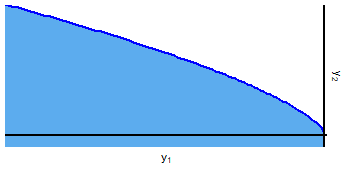
\includegraphics[scale=.75]{problem2a_prodset.png}
		\end{center}
		
	\item[(b)] Let $z=-y_1$ and define $f(z)=Bz^{(2/3)}$. Then,
		\begin{align*}
			\pi(p) 						&= \underset{z}{\text{max }}p_2f(z)-p_1z	\\
			\frac{d\pi}{dz} 			&= p_2f'(z)-p_1 = 0							\\
			\frac{2}{3}Bp_2z^{-1}{3}	&= p_1										\\
			z							&= \left(\dfrac{2Bp_2}{3p_1}\right)^3		\\
			\pi(p)						&= p_2B\left(\left(\dfrac{2Bp_2}{3p_1}\right)^3\right)^{(2/3)}-p_1\left(\dfrac{2Bp_2}{3p_1}\right)^3 
										= \frac{4}{27}B^3\dfrac{p_2^3}{p_1^2}		\\
			Y^*(p)						&= \left( -\left(\dfrac{2Bp_2}{3p_1}\right)^3, B^3\left(\dfrac{2p_2}{3p_1}\right)^2 \right)
		\end{align*}
		
	\item[(c)] We can verify the homogeneity of $\pi(\cdot)$ and $y(\cdot)$ by solving:
		\begin{align*}
			\pi(\lambda p)	&= \frac{4}{27}B^3\dfrac{\lambda p_2^3}{\lambda p_1^2} = \lambda\frac{4}{27}B^3\dfrac{p_2^3}{p_1^2} = \lambda\pi(p)						\\
			Y^*(\lambda p)	&= \left( -\left(\dfrac{2B\lambda p_2}{3\lambda p_1}\right)^3, B^3\left(\dfrac{2\lambda p_2}{3 \lambda p_1}\right)^2 \right) = Y^*(p)
		\end{align*}
		
	\item[(d)]
		\begin{align*}
			 \frac{\partial \pi}{\partial p_1}(p) &= \frac{-8}{27}B^3p_2^3p_1^{-3} = -\left(\dfrac{2Bp_2}{3p_1}\right)^3 = y_1(p)	\\
			 \frac{\partial \pi}{\partial p_2}(p) &= \frac{(4)(3)}{27}B^3p_2^2p_1^{-2} = B^3\left(\dfrac{2Bp_2}{3p_1}\right)^2 = y_2(p)	
		\end{align*}
		
	\item[(e)] 
	\begin{align*}
		D_py(p) &= \begin{pmatrix} \frac{\partial y_1}{\partial p_1} &  \frac{\partial y_1}{\partial p_2} \\  \frac{\partial y_2}{\partial p_1} &  \frac{\partial y_2}{\partial p_2} \end{pmatrix}
				= 
				\begin{pmatrix}  
				\frac{8(Bp_2)^3}{9p_1^4}	& \frac{-8B^3p_2^2}{9p_1^3}  \\  
				\frac{-8B^3p_2^2}{9p_1^3}	&  \frac{8B^3p_2}{9p_1^2} 
				\end{pmatrix} \\
		|D_py(p)| &= \left(\frac{8}{9}\right)^2\frac{B^6p_2^4}{p_1^6} - \left(\frac{8}{9}\right)^2\frac{B^6p_2^4}{p_1^6} = 0 \geq 0	\\
		\frac{\partial y_1}{\partial p_1} &= \frac{8(Bp_2)^3}{9p_1^4} \geq 0 \\
		[D_py]p &= \begin{pmatrix}  
				\frac{8(Bp_2)^3}{9p_1^4}	& \frac{-8B^3p_2^2}{9p_1^3}  \\  
				\frac{-8B^3p_2^2}{9p_1^3}	&  \frac{8B^3p_2}{9p_1^2} 
				\end{pmatrix} \colvec{2}{p_1}{p_2} 
				= \colvec{2}{		\frac{8}{9}\left(\frac{Bp_2}{p_1}\right)^3 		- \frac{8}{9}\left(\frac{Bp_2}{p_1}\right)^3
				}{				-	\frac{8}{9}B^3\left(\frac{p_2}{p_1}\right)^2 	+ \frac{8}{9}B^3\left(\frac{p_2}{p_1}\right)^2
				} = \colvec{2}{0}{0}
	\end{align*}
	
	
\end{itemize}	


%%%________________________________________________________________%%%

\section*{Question 3}
Let $\pi(p)=Ap_1^{-2}p_2^3$, where $A>0$ is known and $p_1,p_2>0$.

\begin{itemize}
	\item[(a)] If $\pi(\cdot)$ is differentiable and convex, then it is rationalizable.
	
	\item[(b)] Suppose $y=(y_1,y_2)\in Y^0$, where $y_2>0$. Then, given the definition of the outer bound,
		\[
			p_2y_2 \leq Ap_1^{-2}p_2^3 - p_1y_1
		\]
		Where $\underset{p_1\rightarrow\infty}{\text{lim }}Ap_1^{-2}p_2^3=0$. Thus, if $p_1$ is arbitrarily large, 
		\[
			p_2y_2 \leq - p_1y_1
		\]
		Where $p_1$, $p_2$, and $y_2$ are all strictly positive. Thus, for this inequality to hold, $y_1$ must be non-negative. In the case of $y_1=0$, then $y_2$ must also equal zero (the shutdown case).
	
	\item[(c)] Starting with the first order condition of the problem, $Y^0$ is derived below by solving $\underset{r}{\text{min }}Ar^2-\frac{y_1}{r}$:
		\begin{align*}
			2Ar + \frac{y_1}{r^2} &= 0		\\
			y_1 &= -2Ar^3					\\
			r &= \sqrt[3]{\dfrac{-y_1}{2A}}	\\
			\therefore 	y_2 &\leq A\left(\frac{-y_1}{2A}\right)^{(2/3)} +(-y_1)\left(\frac{-y_1}{2A}\right)^{-(1/3)} 	\\
						y_2 &\leq A^{\frac{-1}{3}}(-y_1)^{\frac{2}{3}}\left(2^{\frac{-2}{3}}+2^\frac{1}{3}\right)		\\
						y_2 &\leq A^{\frac{-1}{3}}(-y_1)^{\frac{2}{3}}\left(\frac{27}{4}\right)
		\end{align*}
		Thus, the production set encompasses the line $y_2=\frac{27}{4}\sqrt[3]{\dfrac{(-y)^2}{A}}$ and everything below it, for $y_1\leq0$. A visual representation is provided in my answer to question 2(a).
		
	\item[(d)] Let $B=\frac{27}{4}A^{-(1/3)}$ and $z = -y_1$. Then, since profit is increasing on $y_2$, $y_2=\frac{27}{4}\sqrt[3]{\dfrac{(-y)^2}{A}}$, and:
		\[
			\pi(p) = p_2y_2 + p_1y_1 = p_2Bz^{(2/3)} - p_1z
		\]
		Notice that this is the same profit function that was determined in question 2 to have a symmestric and positive semidefifinite Jacobian matrix in question 2, which satisfied the law of supply. Therefore, this profit function would indeed generate the ``data" that we started with.
	
\end{itemize}



%%%________________________________________________________________%%%


\end{document}








